\chapter{Analýza}\label{ch:analysis}
V této kapitole bude probrána specifikace, požadavky na API a také požadavky na celkové fungování hry. Část je také věnována analýze již existujících herních API.

Cílem této práce je vytvořit zdokumentované jednotné API, které bude používáno jak uživatelským prostředím, tak i administrátorským rozhraním.

\section{Analýza již existujících herních API}\label{sec:existing_apis}

Tato část se věnuje představení již existujících online her s evolucí herních situací, která se ukládá mezi sezeními. Těchto her ovšem není mnoho -- většina webových online her nenutí uživatele k přihlášení a také nepodporuje postup či evoluce situací. Takovéto prémiové hry mívají většinou spíše formu desktopových aplikací a v takovém případě by se bohužel špatně analyzovala odcházející a přicházející komunikace.
Byla mi ovšem doporučena jedna hra, která je vytvořená přímo pro hraní za pomocí API, proto jsem se rozhodl tuto hru analyzovat a zjistit, jaké funkce a požadavky by mělo API pro tuto hru splňovat.

\subsection{SpaceTraders API}\label{sub:SpaceTraders}
SpaceTraders je hra založená na REST API, ve které hráči kontrolují a rozšiřují své flotily vesmírných lodí a za jejich pomocí objevují, obchodují a probíjí si vlastní cestu skrz galaxii. Hra je určena pro nadšence, kteří jsou vybízeni vytvořit si vlastní frontend a případně herní mechaniky automatizovat přes jakýkoli jazyk, což může sloužit i jako příjemný nástoj, jak se naučit práci s API nebo nový programovací jazyk. API je zdokumentováno za pomocí technologií OpenAPI a \gls{stoplight}. \cite[]{spacetraders}

Pro dotazování hra využívá jak parametrů dotazu tak proměnných v dotazované URL\@.

Token se vkládá do hlavičky ve formátu \texttt{'Authorization: Bearer INSERT\_TOKEN\_HERE'}. Tento token má formu zakódovaného JWT \sectionref{sec:jwt} objektu pomocí kódování RS256.
Jeho dekódovaný text je zobrazen na obrázku \ref{fig:jwt_spacetraders}.

\begin{figure}[!ht]
    \centering
    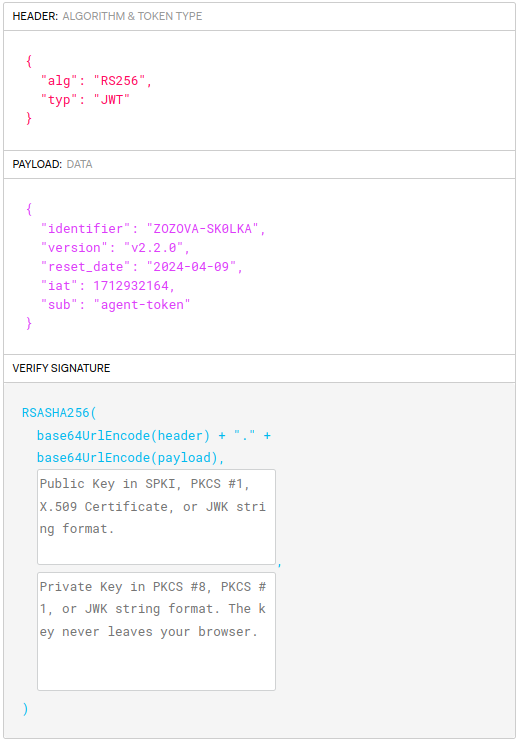
\includegraphics[width=0.5\textwidth]{figures/spaceTraders/jwt.png}
    \caption{Dekódovaný token ze hry SpaceTraders \cite[]{jwt_decoder}}
    \label{fig:jwt_spacetraders}
\end{figure}

Hra nejprve vyžaduje registraci přes endpoint \texttt{/v2/register}. Ten vrátí údaje o novém agentovi spolu s autentizačním tokenem \coderef{code:space_login}[, řádek 3], se kterým se uživatel bude dále ověřovat ve všech následujících požadavcích.

\begin{listing}[!ht]
    \inputminted[breaklines]{json}{resources/code/spaceTraders/login.jsonc}
    \caption{Odpověď na požadavek na registraci\protect\footnotemark}
    \label{code:space_login}
\end{listing}
\footnotetext{Velká část dat musela být pro přehlednost smazána}

Jako odpověď se zde používá formát JSON, který obsahuje především objekt \texttt{data} a poté dodatečné objekty jako třeba \texttt{meta}, ve kterých mohou být další informace jako stránkování. % TODO odkaz na stránkování
Status je použit v souladu s klasickým výkladem statusových kódů % TODO odkaz na ty pravidla někde v restku
a dále je obsahu rozšířen o konkrétní popis chyby v daném požadavku. Příklad je vidět na výpisu \ref{code:space_error}, kde je zobrazena chyba při požadavku na odlet na jinou planetu, neboť loď není na orbitě.


\begin{listing}[ht!]
    \inputminted[breaklines]{json}{resources/code/spaceTraders/error_response.jsonc}
    \caption{Výpis chyby při požadavku odletět na jinou planetu}
    \label{code:space_error}
\end{listing}

\section{Specifikace požadavků}
Pomocí výše provedené analýzy API existujících her, vyčlenění požadavků na funkcionality hry ze strany ostatních členů týmu a za pomocí analýzy dostupných nástrojů pro tvorbu API byly vytyčeny požadavky a funkce, které by mělo API modelové hry podporovat. Jedná se především o CRUD operace se základními objekty, jejich filtrování, stránkování a lazy load. API by taktéž mělo podporovat přihlašování a obranu před základními typy útoků jako je SQL injection, DDOS a DOS útok nebo neoprávněný přístup díky chybám v API.

API by taktéž mělo podporovat validaci všech vstupních dat (rozsahy vstupních hodnot, filtrace speciálních znaků, kontrola správného postupu operací při hraní hry) a mělo by mít odpovídající koncové body pro samotné hraní hry.

\subsection{Funkční požadavky}
Nyní si představíme funkční požadavky na API, které předložili ostatní členové týmu. Tyto požadavky se měnily a rozšiřovaly spolu s průběhem návrhu i implementace. Některé požadavky, které vzešly primárně z backoffice se využívají ve frontendu a případně i naopak.

\subsubsection*{Požadavky, které byly vyčleněny primárně ze strany backoffice}

\begin{enumerate}[label=\textbf{F\arabic*}:, leftmargin=*, align=left]
    \item \textbf{CRUD operace} -- Nad základními objekty, se kterými se bude často pracovat, a upravovat pomocí endpointů. Těmito objekty jsou \texttt{akce, efekty, předměty, charaktery a jejich vlastnosti, dobrodružství, kampaň, obchody, nepřátelé, překážky, lokace} a \texttt{části lokace}
    \item \textbf{Filtrování} -- Možnost vyhledat objekty podle vstupních parametrů u koncových bodů, které poskytují seznam objektů.
    \item \textbf{Lazy load} -- Způsob načítání dat, který umožňuje vracet pouze daný objekt bez jeho závislostí, případně vrácení pouze těch závislostí, které se určí. Výsledkem je rychlejší zpracování a menší objem přesunutých dat, když uživatel tyto závislosti nepotřebuje. Namísto objektu se tedy vrátí jen jeho identifikátor.
    \item \textbf{Stránkování} -- Další způsob předávání dat, který umožní jejich postupné zpracování, což vede ke zkrácení času potřebného k vyhodnocení požadavku jak v API tak ve zobrazovací části.
    \item \textbf{Caching} -- Již jednou zpracovaná data z databáze není třeba znovu získávat z databáze, pokud nedošlo ke změně. Tato funkcionalita umožní násobně rychlejší odezvu pro opakované získávání stejných dat.
    \item \textbf{Administrátorská práva} -- Ne všichni mohou mít přístup pro úpravu dat v databázi. Díky administrátorským přihlašovacím údajům a následnému tokenu se budou moci upravovat a vkládat data do databáze pouze s odpovídajícím ověřením.
    \item \textbf{Validace} -- Data vkládaná do databáze budou validována a případně vrátí chybovou hlášku, podle které bude možno snadno identifikovat chybu vstupních dat a následně ji opravit.
\end{enumerate}


\subsubsection*{Požadavky primárně ze strany uživatelského prostředí}

\begin{enumerate}[label=\textbf{F\arabic*}:, leftmargin=*, align=left]
    \item \textbf{Získávání objektů} -- Bude umožněno získávat jakékoliv objekty, které neobsahují herní data či jiné citlivé informace, přímo z databáze.
    \item \textbf{Podpora herního průběhu} -- Uživatel bude moci projít celým soubojem a interagovat s entitami v něm za pomocí řady validovaných a přehledně uspořádaných koncových bodů.
    \item \textbf{Zamezení zneužití} -- Postup operací v herním průběhu bude kontrolován tak, aby se zamezilo případnému zneužití nebo obcházení pravidel hry.
    \item \textbf{Přihlášení} -- Uživatel se bude moci přihlásit a získat token pro ověření v dalších požadavcích.
    \item \textbf{Herní data} -- Uživatel bude mít pod svým účtem uložený postup hry a bude moci pokračovat tam, kde skončil. Dále bude mít možnost vytvářet nové postavy pro kampaně a také nová dobrodružství.
    \item \textbf{Validace} -- Obsah vstupních dat bude validován a případně vrátí smysluplnou chybovou hlášku.
    \item \textbf{Obrázky} -- Bude možné získat obrázek z url adresy přiložené k objektu, případně v požadavku specifikovat jeho velikost.
\end{enumerate}



\subsection{Nefunkční požadavky}
Dále je důležité vyhradit si nefunkční požadavky. Jejich vznik je stejný jako požadavky funkční, byly sestrojovány postupně s vývojem na základě zkušeností a požadavků ostatních členů týmu.


\begin{enumerate}[label=\textbf{F\arabic*}:, leftmargin=*, align=left]
    \item \textbf{Rozdělení API na dvě části} -- Z důvodu spolupráce na API s jinými členy týmu, především herním systémem, který pro svůj chod využívá stejných modelů, bylo rozhodnuto, že herní logika i mapování bude v jednom projektu. Tomu tedy musí být přizpůsobena i spolupráce a podpůrné technologie.
    \item \textbf{Dokumentace} API bude zdokumentováno za pomocí OpenAPI a pro vizuální zobrazení koncových bodů bude použit Swagger, který zároveň poslouží jako skvělé ladící rozhraní.
    \item \textbf{Hosting} API bude stejně jako ostatní části projektu hostováno na veřejných serverech.
    \item \textbf{Přehlednost} Koncové body API by měly být samopopisující a snadno pochopitelné.
    \item \textbf{Standardizovanost} API se bude držet ověřených dobrých praktik z praxe a bude udržovat jednotnost a standardizovanost.
\end{enumerate}

\section{Uložení dat}\label{sec:data_storage}
Pro ukládání dat existuje mnoho různých databázových systémů, ať už relační nebo dokumentové. v této kapitole budou probrány možnosti výběru databáze pro hru.

\subsection{SQL database}\label{sec:data_storage:relational_db}
Relační databáze, jindy nazývané \gls{sql} databáze, jsou databáze, které využívají strukturovaných dotazů (\gls{sql}) pro manipulaci dat. Data jsou reprezentována tabulkami, které mají předdefinovány relace mezi ostatními tabulkami. Je to nejčastěji používaný styl databáze. Nejlépe se hodí pro strukturovaná data. Jedny z nejpoužívanějších relačních databází jsou \textbf{MySQL}, \textbf{PostgreSQL} a \textbf{SQLite}.\cite{guidetochoosingdatabase}\cite{howtochoosedatabase}

Při použití \gls{rdbms} chráníme svá data před ztrátou a díky ACID vlastnostem máme jistotu o konzistenci dat. Nyní níže budou popsány jednotlivé vlastnosti ACID.\label{sec:data_storage:relational_db:ACID}\cite{acidvsbase}

\textbf{Atomičnost} zajišťuje, že se všemi transakcemi je zacházeno jako s jedním celkem. Jediné dvě možnosti jak transakce může dopadnout je buď celá úspěšně a nebo celá neúspěšně. Když se transakce skládá z více částí, majoritní část se provede tak provedené operace v transakci se vrátí do původní podoby.

Díky \textbf{konzistenci} budou do databáze vložena pouze validní data. Pokud vstupní data nejsou validní, databáze se vrátí do původní podoby. Díky tomu se předejde poškození databáze.

\textbf{Izolace}  zajišťuje, že nedokončené transakce nebudou ovlivněny jinými transakcemi. Díky této vlastnosti může jednoduše pracovat na databázi více uživatelů najednou bez ovlivnění se navzájem.

\textbf{Durabilita} znamená, že uložená data nebudou ztracena ani když transakce selže nebo když dojde k výpadku systému.

Mezi hlavní nevýhody relačních databází je nízká flexibilita neboli neefektivnost pracovat s nestrukturovanými daty, takže se nedají dobře použít na Internet of Things aplikace. S neflexibilitou se pojí špatný návrh pro komplexní datové struktury. Taky relační databáze se nemohou škálovat do šířky, neboli zátěž se nemůže rozložit na více serverů.

\subsection{noSQL database}\label{sec:data_storage:noSQL}
Dokumentové databáze umožňují ukládání a zpracovávání nestrukturovaných dat (hudba, fotografie, atd.), což umožňuje vývojářům mít větší flexibilitu nad daty, což je jedna z největších výhod dokumentových databází. Taktéž se mohou škálovat do šířky, takže zpracování velkého množství dat není obtížné. Mají taktéž velkou toleranci proti chybám. S velkou tolerancí chyb se pojí limitované ACID vlastnosti, kdy místo ACID využívají BASE vlastnosti, které jsou popsány níže. Tyto databáze nemají unifikovaný dotazovací jazyk jako relační databáze a mohou mít problém s komplexními dotazy. Nejčastěji používané dokumentové databáze jsou \textbf{MongoDB} a \textbf{CouchDB}.\cite{guidetochoosingdatabase}\cite{howtochoosedatabase}

\textbf{BASE}\label{sec:data_storage:base} je zkratka pro \textbf{Basically Available}, což znamená že databáze bude dostupná pro uživatele za všech okolností. neboli uživatel nemusí čekat než jiný uživatel dokončí svou transakci. \textbf{Soft state} znamená, že data se mohou nacházet v temporálním stavu když běží více transakcí zároveň a můžou se změnit i po dokončení transakce. Data přejdou do finálního stavu až když jsou všechny transakce dokončeny. S tím se pojí \textbf{Eventually consistent}, kdy data se dostanou do konzistentního stavu po všech souběžných aktualizacích. V tento moment všechny aplikace vidí stejná data.\cite{acidvsbase}

\subsection{Porovnání SQL a noSQL databází}

V tabulce \ref{tab:sql_vs_nosql} máme přehledně porovnány vlastnosti SQL a noSQL databází. Pro naše použití jsme vybrali že bude vhodnější SQL databáze díky reprezentaci jedna tabulka v databázi = jeden objekt v API. Taktéž jsme všichni již pracovali s SQL databázemi a vedoucím práce nám byla doporučena SQL databáze. Přechod na noSQL by bylo zabředávání do neznámých vod.

\begin{table}
    \centering
    \begin{tabular}{|l|l|l|}
        \hline
        kritérium        & SQL               & noSQL            \\
        \hline
        Typ dat          & Strukturovaná     & Nestrukturovaná  \\
        Flexibilita      & Nízká             & Vysoká           \\
        Škálovatelnost   & Vertikální        & Horizontální     \\
        Schéma           & Striktní          & Dynamické        \\
        Transakce        & ACID              & BASE             \\
        Dotazovací jazyk & SQL               & Není unifikovaný \\
        Příklady DB      & PostgreSQL, MySQL & MongoDB, Redis   \\
    \end{tabular}
    \caption{Porovnání SQL a noSQL databází}\label{tab:sql_vs_nosql}
\end{table}

Nyní si představíme nejznámější SQL databáze.

\subsection{MySQL}\label{sec:data_storage:mysql}
MySQL je jedna z nejpoužívanějších databází. Má velkou podporu a je open-source, funguje velmi dobře s většinou knihoven a frameworků. Skvěle se hodí na menší až střední projekty. Obsahuje komplexní sadu funkcionalit jako jsou triggery, procedury, pohledy a podpora transakcí. Ve větších projektech může mít problémy s výkonem  a s komplexními dotazy.\cite{guidetochoosingdatabase}\cite{howtochoosedatabase}


\subsection{PostgreSQL}\label{sec:data_storage:postgresql}
Tato databáze je objektově relační což je podobné jako relační jen data jsou ukládány v objektech místo tabulek jako je tomu například u MySQL. Přednosti PostgreSQL jsou pokročilé indexování, vlastní datové typy , komplexní dotazy a cizí klíče, a dovoluje volat procedury napsané v jiném jazyce než SQL. Nicméně je náročnější na výkon, některé vlastnosti mohou být náročné na nakonfigurování a může být pomalejší při čtení dat.\cite{guidetochoosingdatabase}\cite{howtochoosedatabase}

\subsection{Výběr databáze}\label{sec:data_storage:summary}
Nakonec jsme vybrali primárně díky doporučení našeho vedoucího práce MariaDB, což je založeno na MySQL. MariaDB je osamocená větev původních vývojářů, po tom co MySQL bylo získáno společností Oracle. Je rychlejší, podporuje \textit{neviditelné sloupce} a má propracovanější views.

\section{Technologie pro tvorbu API}\label{sec:api_technologies}
v této kapitole bude probráno jaké frameworky a technologie jsou dostupné pro tvorbu API. Níže je výčet těch nejznámějších a nejpoužívanějších s ohledem na požadavky a zkušenosti týmu.

\subsection{Spring Boot}\label{sec:api_technologies:spring}
% \begin{wrapfigure}{r}{0.3\textwidth} % TODO idk jestli tu dávat obrázky
%     \centering
%     
\includegraphics[width=0.2\textwidth]{figures/logos/springboot.png}
%     \caption{Logo Spring Bootu, zdroj: } %%TODO kdyžtak to dát do cite \url{https://www.pngaaa.com/detail/2459546}
%     \label{fig:spring}
% \end{wrapfigure}
Založen originálně na Spring technologii ale snaží se udělat originální Spring framework více uživatelsky přívětivý. Spring boot obsahuje v sobě vše, co je třeba, bez velkého konfigurování knihoven. Je určen i pro velké aplikace ve velkých společnostech jako je Netflix. Kromě programovacího jazyku Java podporuje i Kotlin a Groovy. Má velkou podporu komunity a skvělou dokumentaci. Ovšem může být náročnější na hardware a binární soubory jsou větší kvůli velkému množství knihoven.

\subsection{ASP.NET Core}\label{sec:api_technologies:asp}
Uzavřený framework od Microsoftu, který je určen pro webové aplikace. Jedná se o alternativu ke Springu u Javy ovšem pro jazyk C\#. Je zde navíc lepší podpora asynchronních operací a je zde \gls{linq}. Oproti Springbootu má i vlastní ekosystém nástrojů jako je třeba microsoft Azure nebo MSSql databáze. ASP.NET Core i Spring boot jsou velmi solidní frameworky i pro velké firmy a vyloženě záleží na preferenci programovacího jazyka.

\subsection{Django REST}\label{sec:api_technologies:django}
Založeno na Django frameworku a jeho pohledech založených na třídách \textit{class-based views}. Celkově se jedná o velice bezpečný framework určený pro programovací jazyk Python, s rychlou učící křivkou a s obsáhlou dokumentací. Ovšem u větších projektů je méně přehledný než výše zmíněné frameworky.

\subsection{Fast API}\label{sec:api_technologies:fast}
Jakožto alternativu k Djangu zde máme Fast API, kde je plně podporováno asynchronní programování a je přímo určeno pro vývoj RESTful API. Je taktéž pro Python, je velmi rychlý jak na naučení tak i framework jako takový a je plně otypovaný oproti Djangu. Má dobrou dokumentaci a mezi vývojáři je čím dál populárnější. Ovšem má horší validaci vstupních dat.


\subsection{Výběr frameworku}\label{sec:api_technologies:summary}
Pro účely RESTful API byl výběr očividný, Fast API které je navrhnuto pro rychlou tvorbu RESTful API a pro vývojáře velice příjemným otypováním. Je taktéž jeden z nejrychlejších Python frameworků v některých věcech na úrovní například Spring bootu.\cite{benchmarks} Taktéž Python je jeden z jednodušších jazyků a všichni členové týmu už s ním mají zkušenosti. Ovšem později se na doporučení přešlo na Spring boot díky jeho jednoduššímu \gls{orm} a větší přehlednosti.